\documentclass[10pt]{beamer}
\usepackage[slovene]{babel}
\usepackage[utf8]{inputenc}
\usepackage[T1]{fontenc}
\usepackage{mathptmx}
\usepackage{helvet}
\usepackage{courier}
\usepackage{hyperref}
\usepackage{wrapfig}
\usepackage{tikz}
\usepackage{tcolorbox}
\usepackage{amsmath,amssymb,amsfonts}
\usepackage{graphicx}


\usetheme{Madrid}

\begin{document}

\title[Finančni instrumenti osnovani na razpršenosti]{Finančni instrumenti osnovani na razpršenosti}
\author[Žan Jarc]{Žan Jarc \\[0.5cm] \footnotesize Mentorica: prof. dr. Damjana Kokol Bukovšek \\[0.3cm] Somentor: dr. Aleš Toman}

\institute [FMF]{ Fakulteta za matematiko in fiziko}

\begin{frame}
	\titlepage
\end {frame}

\begin{frame}
\textbf{Vsebina predstavitve}:
	\begin{itemize}
		\item Volatilnost trga
		\item Indeks Standard \& Poor’s~500
		\item Indeks volatilnosti
		\item Primer izračuna indeksa VIX
		\item Primerjava vrednosti indeksov S\&P 500 in VIX
		\item VIX terminske pogodbe
		\item VIX opcije
	\end{itemize}
\end {frame}

\begin{frame}
\frametitle{Volatilnost trga (1)}
\begin{itemize}
\item \textbf{Finančni trg} sestavljajo vrednostni papirji, katerih vrednosti se v času spreminjajo.
\item Zaradi spreminjanja vrednosti vsak vrednostni papir ali pa portfelj papirjev ustvarja donose in izgube.
\item Če donos ali izgubo delimo z začetno vrednostjo papirja ali portfelja, temu rečemo \textbf{donosnost}, ki je izražena v odstotkih in je lahko pozitivna ali negativna.
\item  Razpršenost donosnosti je lahko večja ali manjša. Standardnemu odklonu porazdelitve donosnosti rečemo \textbf{volatilnost}.

\end{itemize}
\end{frame}

\begin{frame}
\frametitle{Volatilnost trga (2)}
\begin{itemize}
\item Investitorji lahko s pomočjo informacije o volatilnosti potencialne naložbe ugotovijo, kako tvegana je njihova investicija.
\item  Pri vlaganju v finančno naložbo z nizko volatilnostjo se pričakuje, da bodo donosi investicije morda nizki, vendar precej netvegani, medtem ko nam lahko investicija v finančno naložbo z visoko volatilnostjo prinese višje donose, vendar tudi večje tveganje.
\item Finančni inštrumenti na osnovi volatilnosti so bili zasnovani, da vlagateljem ponudijo možnost, da trgujejo z razpršenostjo in s tem zavarujejo svoj portfelj pred nenadnimi nihaji.
\end{itemize}

\end{frame}

\begin{frame}
\frametitle{Izračun indeksa Standard \& Poor’s~500}
\begin{itemize}
\item \textbf{Indeks Standard \& Poor's~500} ali indeks \textbf{S\&P~500} je pokazatelj stanja v ameriškem gospodarstvu, ki se najpogosteje uporablja.
\item Je kapitalizacijsko utežen indeks: 
$$
\text{S\&P~500} = \sum_{i=1}^{500}\frac{P_i \cdot{} Q_i}{D},
$$
\item  \textbf{$P_i$} cena delnice $i$-tega podjetja.
\item  \textbf{$Q_i$} število razpoložljivih delnic za trgovanje $i$-tega podjeta.
\item  Pri izračunu uporablja tudi delitelj $D$ (angl. \textit{divisor}).

\end{itemize}
\end{frame}

\begin{frame}
\frametitle{Opcije na vrednost indeksa S\&P 500}
\begin{itemize}
\item Indeks S\&P~500 ni le uporaben za reprezentacijo ameriškega gospodarstva ampak tudi predstavlja dobro dolgoročno investicijo.
\item Direktno v indeks ne moremo investirati, lahko pa izoblikujemo portfelj delnic, ki je ekvivalenten sestavi indeksa.
\item Kratica SPX.
\item Je denarno poravnana opcija in je evropskega tipa.
\item Tedenske in mesečne opcije.
\item Pogodbeni množitelj 100 \$.
\end{itemize}

\end{frame}



\begin{frame}
\frametitle{Vrednosti indeksa S\&P 500}
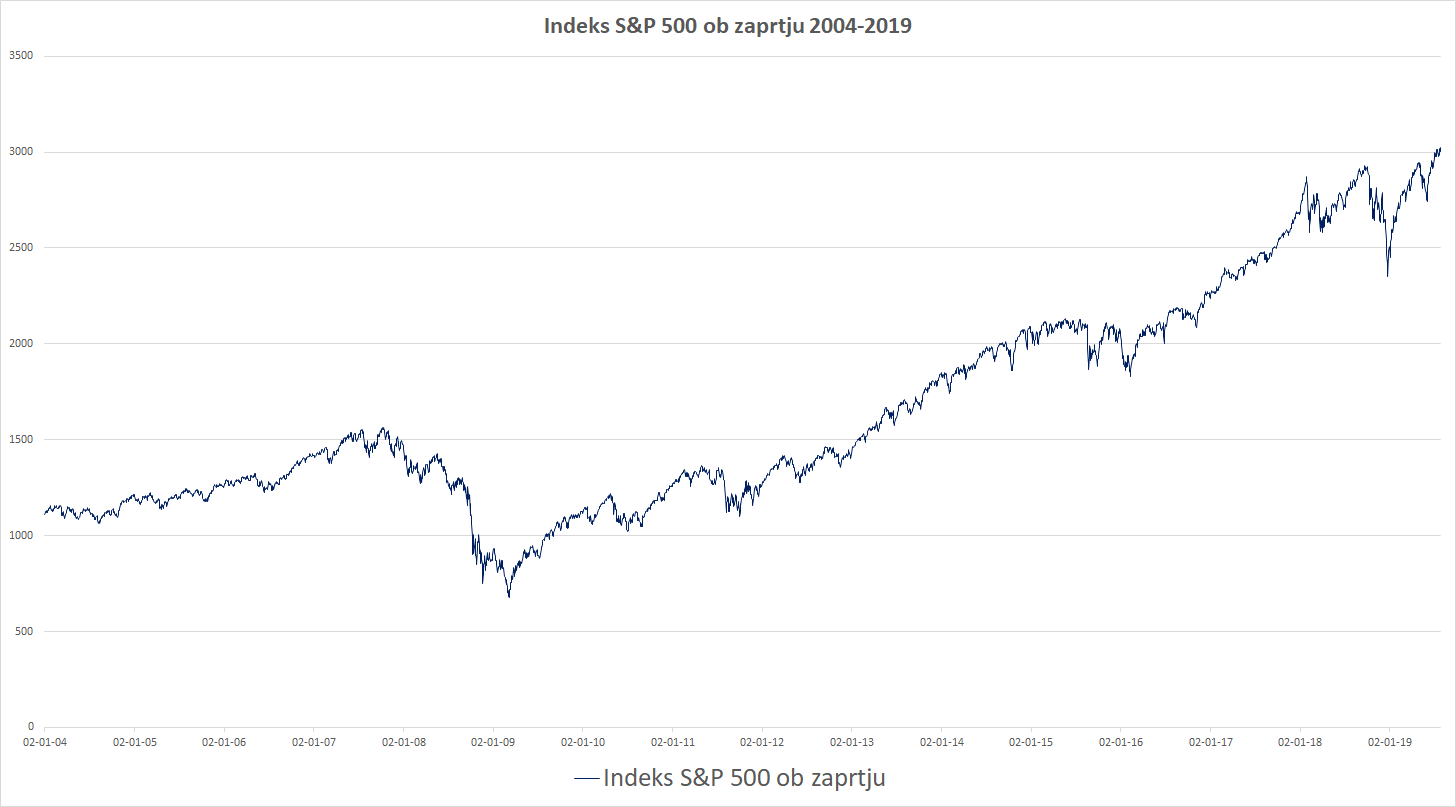
\includegraphics[width=1\textwidth]{./Grafi/SPX_2004-2019.png}
\end{frame}



\begin{frame}
\frametitle{Indeks volatilnosti}
\begin{itemize}
\item Indeks \textbf{Cboe Volatility Index} ali \textbf{VIX} je bil razvit za napovedovanje pričakovane volatilnosti.
\item Indeks prikazuje 30 dnevno pričakovano volatilnost nakupnih in prodajnih opcij na indeks S\&P 500, ki se ne splačajo (angl. \textit{out-of-the-money}) in ki zapadejo čez več kot 23 in manj kot 37 dni. 
\item Odraža pričakovanje investitorjev, kako bo trg nihal v prihodnjih 30 dneh.
\end{itemize}
\end{frame}

\begin{frame}
\frametitle{Primer izračuna indeksa VIX (1)}
\begin{itemize}
\item Izračun vrednosti indeksa VIX na dan 4. marca 2020.
\item Vrednost indeksa S\&P~500 je bila na ta dan 3089,78, vrednost indeksa VIX pa 31,99.	
\item Zaradi lažje preglednosti, uporabimo za izračun le opcije na vrednost indeksa S\&P~500, ki zapadejo čez 27 ali 31 dni.
\end{itemize}
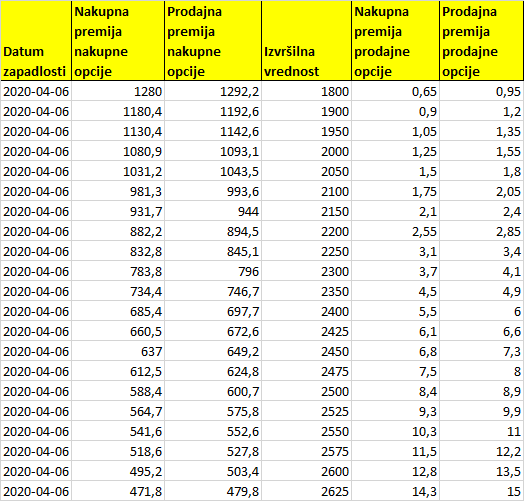
\includegraphics[width=1\textwidth]{./Grafi/Opcije_clean.png}


\end{frame}


\begin{frame}
\frametitle{Primer izračuna indeksa VIX (2)}
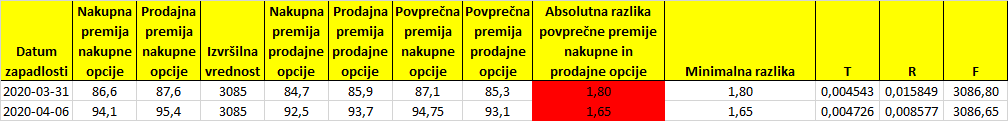
\includegraphics[width=1\textwidth]{./Grafi/Opcije_min_diff.png}
\begin{itemize}
\item $T$ \textbf{čas zapadlosti}
$$
T = \frac{ M_{\text{današnji dan}} + M_{\text{dan poravnave}} + M_{\text{ostali dnevi}}}{\text{ minute v letu}},
$$
\item $R$ \textbf{netvegana obrestna mera} glede na krivuljo donosnosti ameriških zakladnih obveznic
\item $F$ \textbf{terminska vrednost indeksa, določena na osnovi premij indeksnih opcij}
$$
F=K \cdot e^{RT} \cdot (c-p)
$$
\item Za vsak dan zapadlosti opcij določimo $K_0$, ki je prva izvršilna vrednost opcije, manjša ali enaka od izračunane vrednosti $F$ za tisti dan.

\end{itemize}


\end{frame}


\begin{frame}
\frametitle{Primer izračuna indeksa VIX (3)}
\begin{itemize}
\item Pri izbiri nakupnih opcij, ki bodo uporabljene za izračun indeksa VIX, so primerne le tiste z izvršilno vrednostjo večjo ali enako $K_0$. Najprej se izberejo tiste nakupne opcije, ki imajo izvršilno vrednost takoj nad $K_0$. Nadaljujemo iskanje primernih nakupnih opcij z višjo izvršilno vrednostjo, ki imajo nakupno premijo večjo od 0. Ko se pri iskanju pojavita dve zaporedni opciji z nakupno premijo enako nič, se iskanje konča in nobena nakupna opcija z višjo izvršilno vrednostjo ni vključena za izračun indeksa.
\end{itemize}
\begin{center}
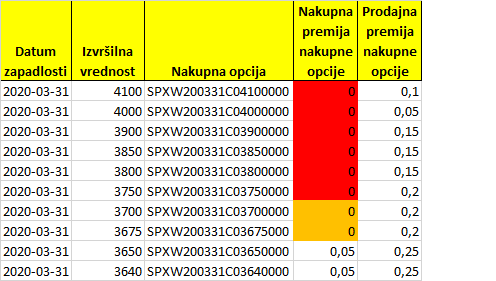
\includegraphics[width=0.65\textwidth]{./Grafi/Calls_T1_clean.png}
\end{center}
\end{frame}


\begin{frame}
\frametitle{Primer izračuna indeksa VIX (4)}
\begin{itemize}
\item Podoben postopek se opravi tudi za iskanje primernih prodajnih opcij, le da se pri tem iskanju upošteva le opcije z izvršilno vrednostjo manjšo ali enako $K_0$. V izračun se vključijo najprej tiste prodajne opcije, ki imajo izvršilno vrednost takoj pod $K_0$ in nato še vse ostale z nižjo izvršilno vrednostjo in nakupno premijo večje od 0. Kot pri izbiri nakupnih opcij, se iskanje prodajnih opcij za izračun indeksa končna, ko se pri razvrščanju naleti na dve zaporedni prodajni opciji, z nakupno premijo enako 0.
\end{itemize}
\begin{center}
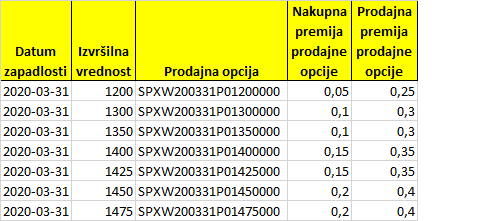
\includegraphics[width=0.7\textwidth]{./Grafi/Puts_T1_clean.png}
\end{center}
\end{frame}


\begin{frame}
\frametitle{Primer izračuna indeksa VIX (5)}
\begin{itemize}
\item S tem postopkom so izbrane vse prodajne in nakupne opcije, ki bodo upoštevane pri izračunu indeksa VIX.\\

\item Za $i$-to opcijo z  izvršilno ceno $K_i$ določimo $\operatorname{\Delta}K_i$ kot:
$$
\Delta K_i = \frac{K_{i+1} - K_{i-1}}{2}
$$
\item Za vsak čas zapadlosti $T_j$ izračunamo $\sigma_j^2$:
$$
\sigma_j^2 = \frac{2}{T_j}\sum_{i}{}\frac{\Delta K_i}{K_i^2}e^{R_jT_j}Q(K_i) - \frac{1}{T_j}\bigg(\frac{F_j}{K_0} - 1\bigg)^2, \quad \text{za}\  j = {23,\ 24, \dots,\ 37},
$$
kjer je $Q(K_i)$ povprečje nakupne in prodajne premije $i$-te opcije.
\end{itemize}
\end{frame}


\begin{frame}
\frametitle{Primer izračuna indeksa VIX (6)}
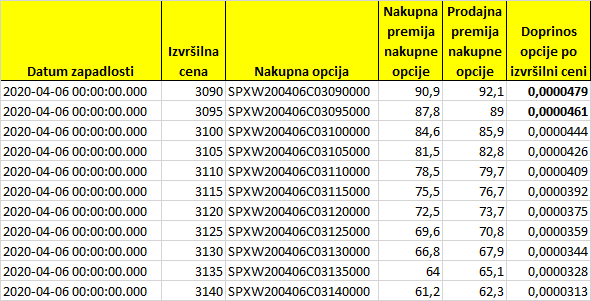
\includegraphics[width=1\textwidth]{./Grafi/Option_contribution.png}
$$
\sigma_1^2 = 1,511730404,\ \sigma_2^2 = 1,677280934
$$

\end{frame}


\begin{frame}
\frametitle{Primer izračuna indeksa VIX (7)}
\begin{itemize}
\item Za končni izračun indeksa VIX moramo izračunati 30-dnevno uteženo povprečje $\sigma_j^2$:
$$
\text{VIX} = 100 \cdot \sqrt{\frac{1}{N_{37}-N_{23}}\Bigg\{ \sum_{j=23}^{37}T_j\sigma_j^2\left\lvert N_j - N_{\text{mesec}}\right\rvert \Bigg\}\cdot \frac{N_\text{{leto}}}{N_{\text{mesec}}}},
$$
kjer je:
\item $N_j$ število minut do zapadlosti opcije, ki zapade čez $j$ dni
\item $N_{\text{leto}}$ število minut v letu ($365\cdot1440=525.600$)
\item $N_{\text{mesec}}$ število minut v mesecu ($30\cdot1440=43.200$)
\end{itemize}

\end{frame}


\begin{frame}
\frametitle{Primer izračuna indeksa VIX (8)}
Za poenostavljen zgled lahko izračnamo indeks VIX kot:
$$
\text{VIX} = 100 \cdot \sqrt{\frac{1}{N_{37}-N_{23}}\Bigg\{T_1\sigma_1^2\left\lvert N_{27} -N_{\text{mesec}}\right\rvert  + T_2\sigma_2^2\left\lvert N_{31} -N_{\text{mesec}}\right\rvert \Bigg\}\cdot \frac{N_\text{leto}}{N_{\text{mesec}}}}
$$
$$
\text{VIX} = 30,84
$$
\end{frame}


\begin{frame}
\frametitle{Primerjava vrednosti indeksov S\&P 500 in VIX (1)}
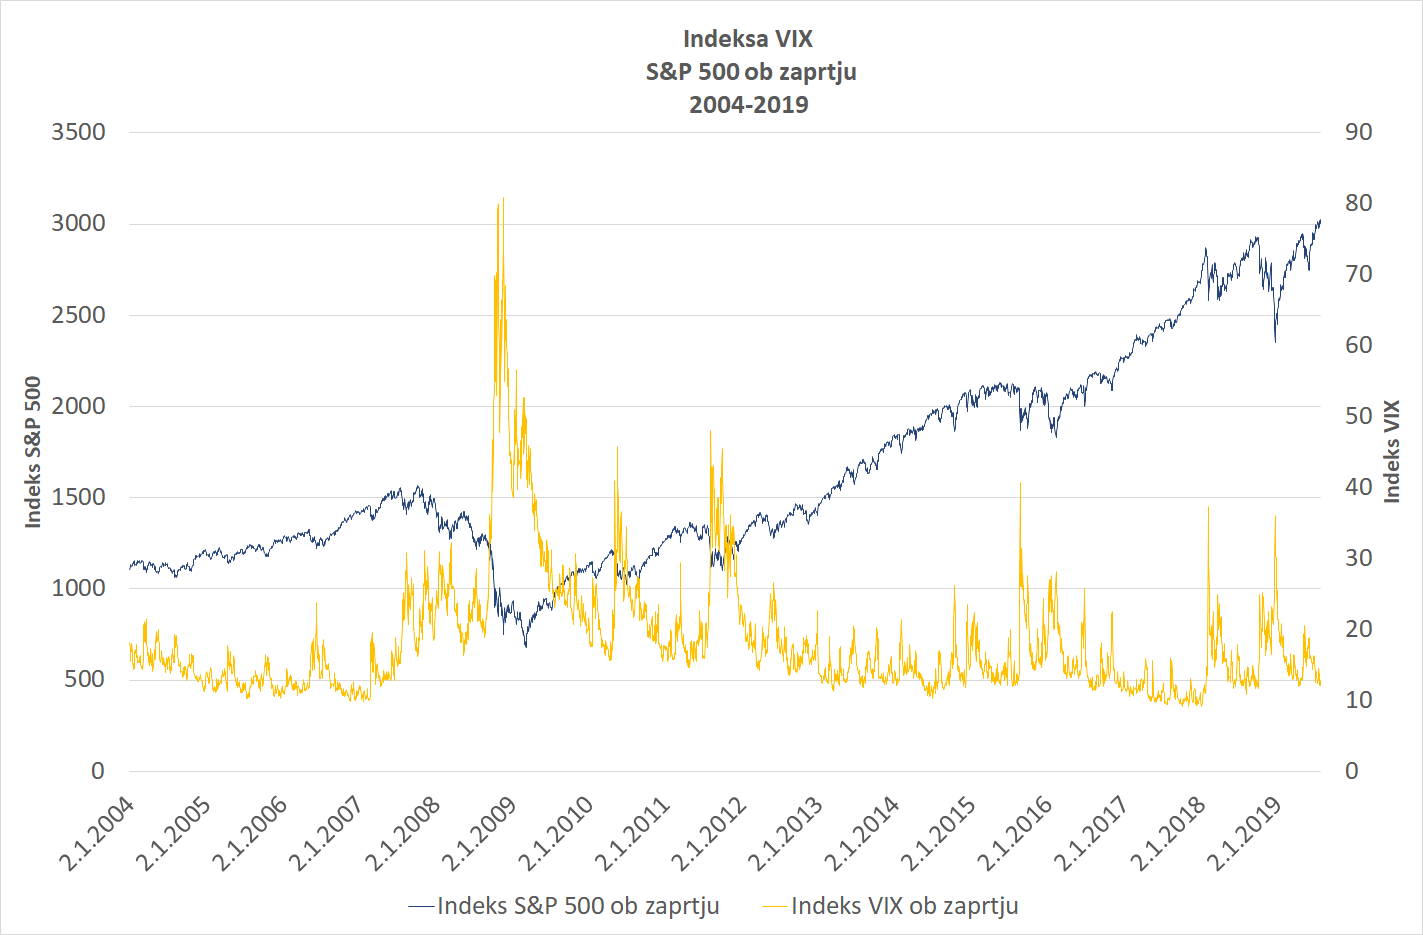
\includegraphics[width=1\textwidth]{./Grafi/VIX_vs_SPX_2004-2019.png}
\end{frame}


\begin{frame}
\frametitle{Primerjava vrednosti indeksov S\&P 500 in VIX (2)}
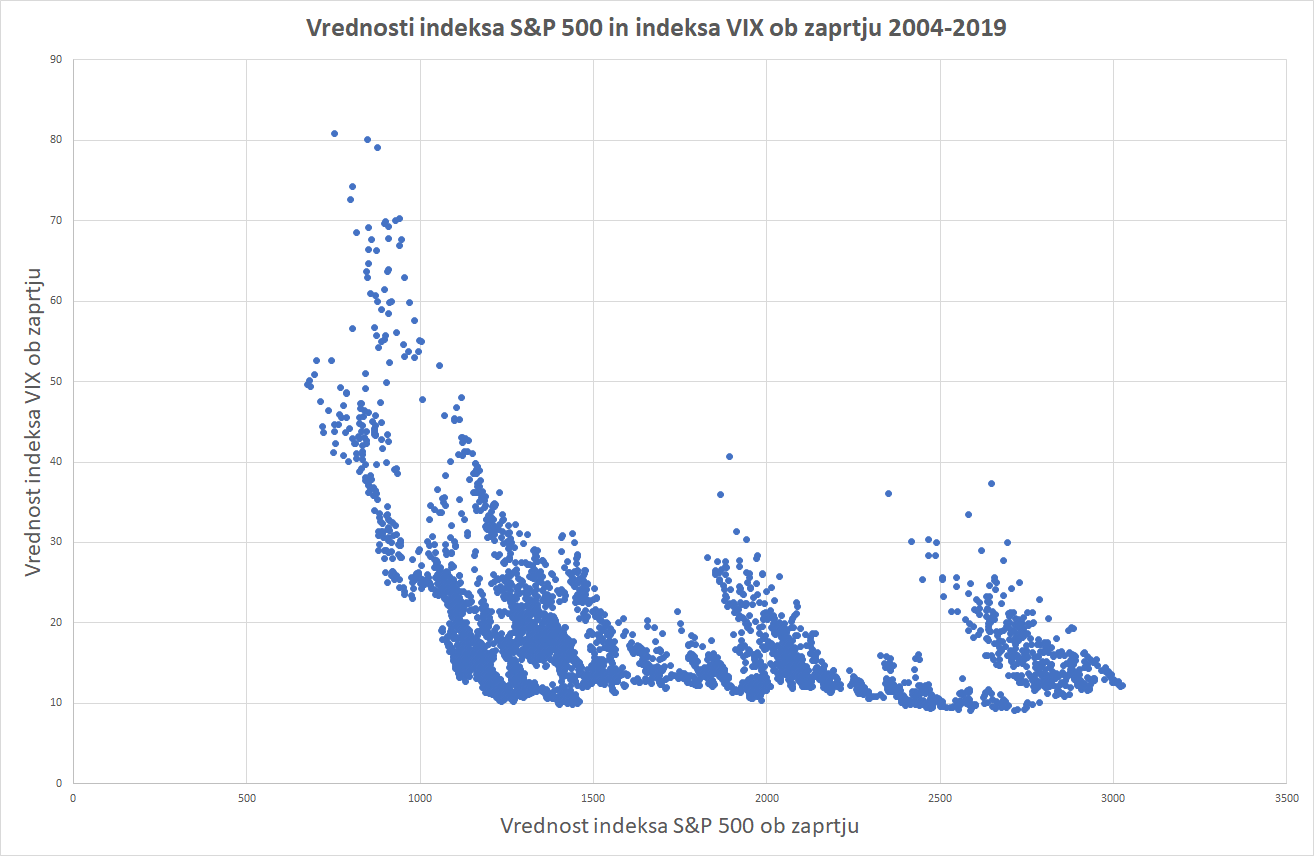
\includegraphics[width=1\textwidth]{./Grafi/VIX_vs_SPX.png}
\end{frame}


\begin{frame}
\frametitle{Primerjava vrednosti indeksov S\&P 500 in VIX (3)}
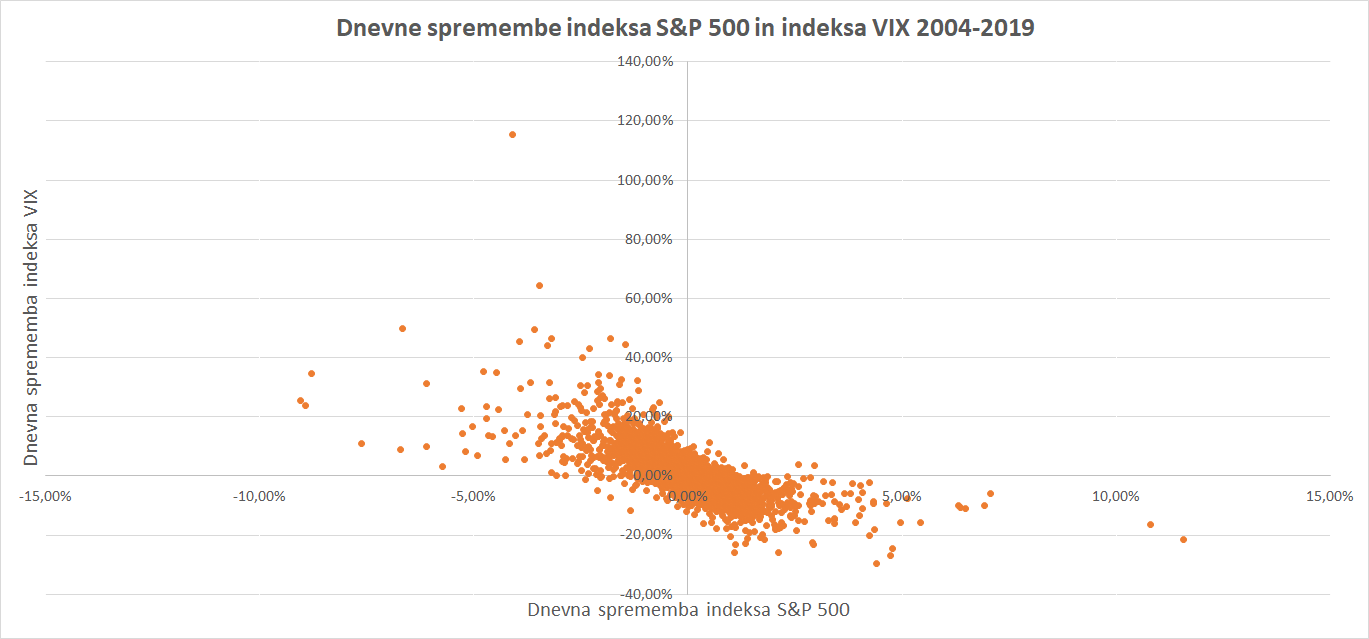
\includegraphics[width=1\textwidth]{./Grafi/VIX_scatter.png}
\end{frame}


\begin{frame}
\frametitle{VIX terminske pogodbe}
\begin{itemize}
\item VIX terminske pogodbe (angl. \textit{VIX futures}) so bili prvič predstavljeni leta 2004 in jih lahko najdemo pod oznako VX (mesečne terminski pogodbe) in VX01 do VX53 (tedenske terminski pogodbe).Izvršilne vrednosti terminske pogodbe z bližanjem ročnosti konvergirajo k vrednosti VIX.
\item Pogodbeni množitelj 1000 \$.
\item Terminske pogodbe imajo ročnost na sredo \textbf{zjutraj}, ki je 30 dni pred petkom, ko zapadejo SPX opcije.
\item Vrednost indeksa, s katero se določi znesek ni določen z vrednostjo indeksa VIX na dan poravnave, temveč z vrednostjo \textbf{volatility index settlement - VRO} (angl. \textit{Special Opening Quotation}). 


\end{itemize}
\end{frame}


\begin{frame}
\begin{itemize}
\frametitle{Opcije na vrednost indeksa VIX}
\item VIX opcije so bile prvič na voljo leta 2006 in jih najdemo pod kratico VIX.
\item  Opcije so evropske in so denarno poravnane.
\item Pogodbeni množitelj 100 \$.
\item Imajo podobno kot terminske pogodbe, ročnost na sredo, ki je 30 dni pred petkom, ko zapadejo opcije na vrednost indeksa S\&P 500.
\item Vrednost opcij VIX je vezana na VIX terminski posel z enako ročnostjo in ne na vrednost indeksa VIX.


\end{itemize}

\end{frame}
\end{document}


















\end{document}